% arara: pdflatex: { shell: true, draft: true }
% arara: makeglossaries
% arara: biber
% arara: pdflatex: { shell: true, synctex: true }
% arara: pdflatex: { shell: true, synctex: true }

\documentclass[12pt,DIV14,BCOR10mm,a4paper,twoside,parskip=half-,headsepline,headinclude,english,ngerman,bibliography=totocnumbered]{scrreprt}

\usepackage{hshhelper_base}

%%%%%%%%%%%%%%%%%%%%%%%%%%%%%%%%%%%%%%%%%%%%%%%%%%%%%%%%%%%%%%%%%%%%%%%%%%
\begin{document}    % hier gehts los
  \thispagestyle{empty} % Titelseite

\includegraphics[width=0.2\textwidth]{Wortmarke_WI_schwarz}

   {  ~ \sffamily
  \vfill
  {\Huge\bfseries Test-Driven-Development in Scrum}
  \bigskip

  {\Large
  Dennis Grabowski \\[2ex]
  Projekt- \& Qualitätsmanagement \\
  Wintersemester 18/19
 \\[5ex]
   \today }
}
 \vfill

  ~ \hfill
  
\includegraphics[height=0.3\paperheight]{H_WI_Pantone1665}

\vspace*{-3cm}

\tableofcontents  % Inhaltsverzeichnis

\chapter{Einleitung}
\chapter{Test-Driven-Development}

\begin{figure}[!htb]
  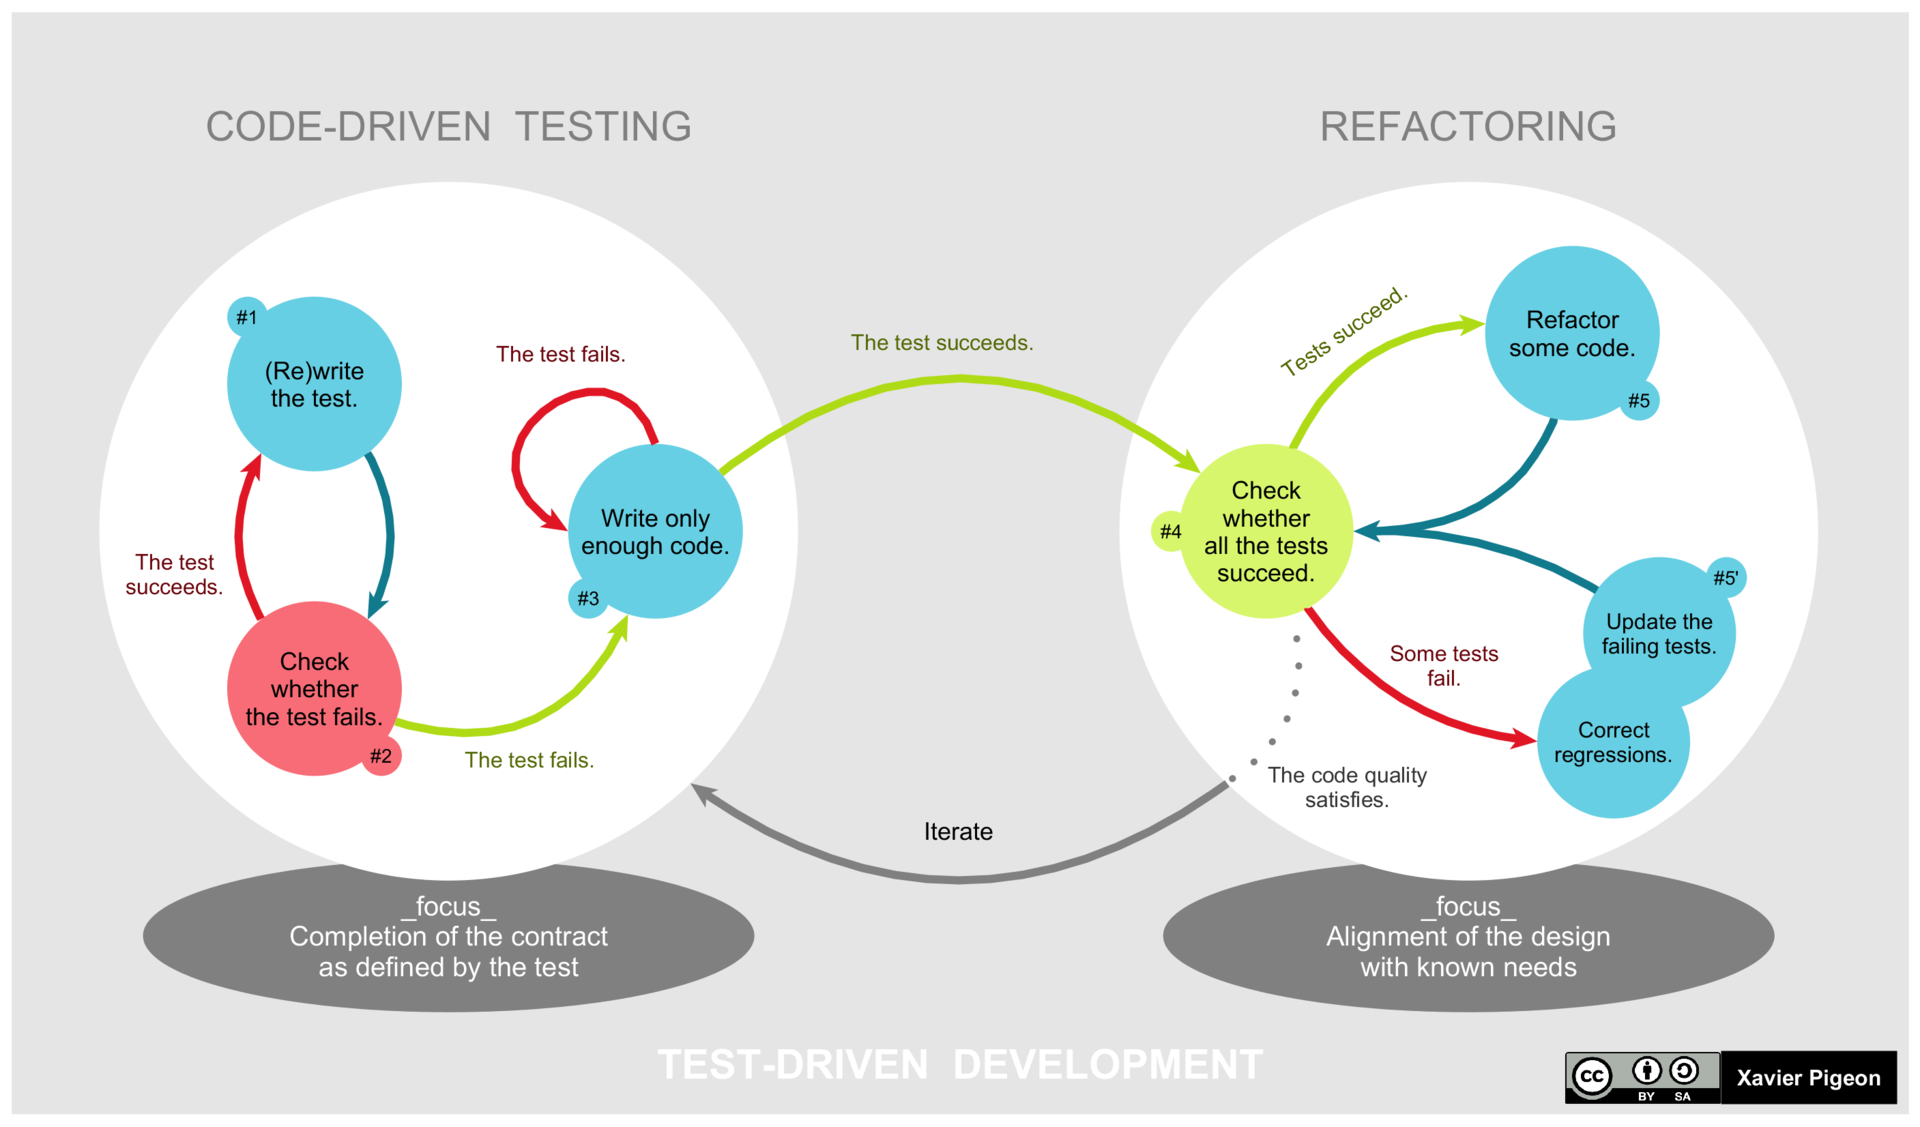
\includegraphics[width=\textwidth,height=0.85\textheight,keepaspectratio]{./images/1920px-TDD_Global_Lifecycle.png}
\autocite{TDD.Picture}
\end{figure}

\chapter{Scrum}

\begin{figure}[!htb]
  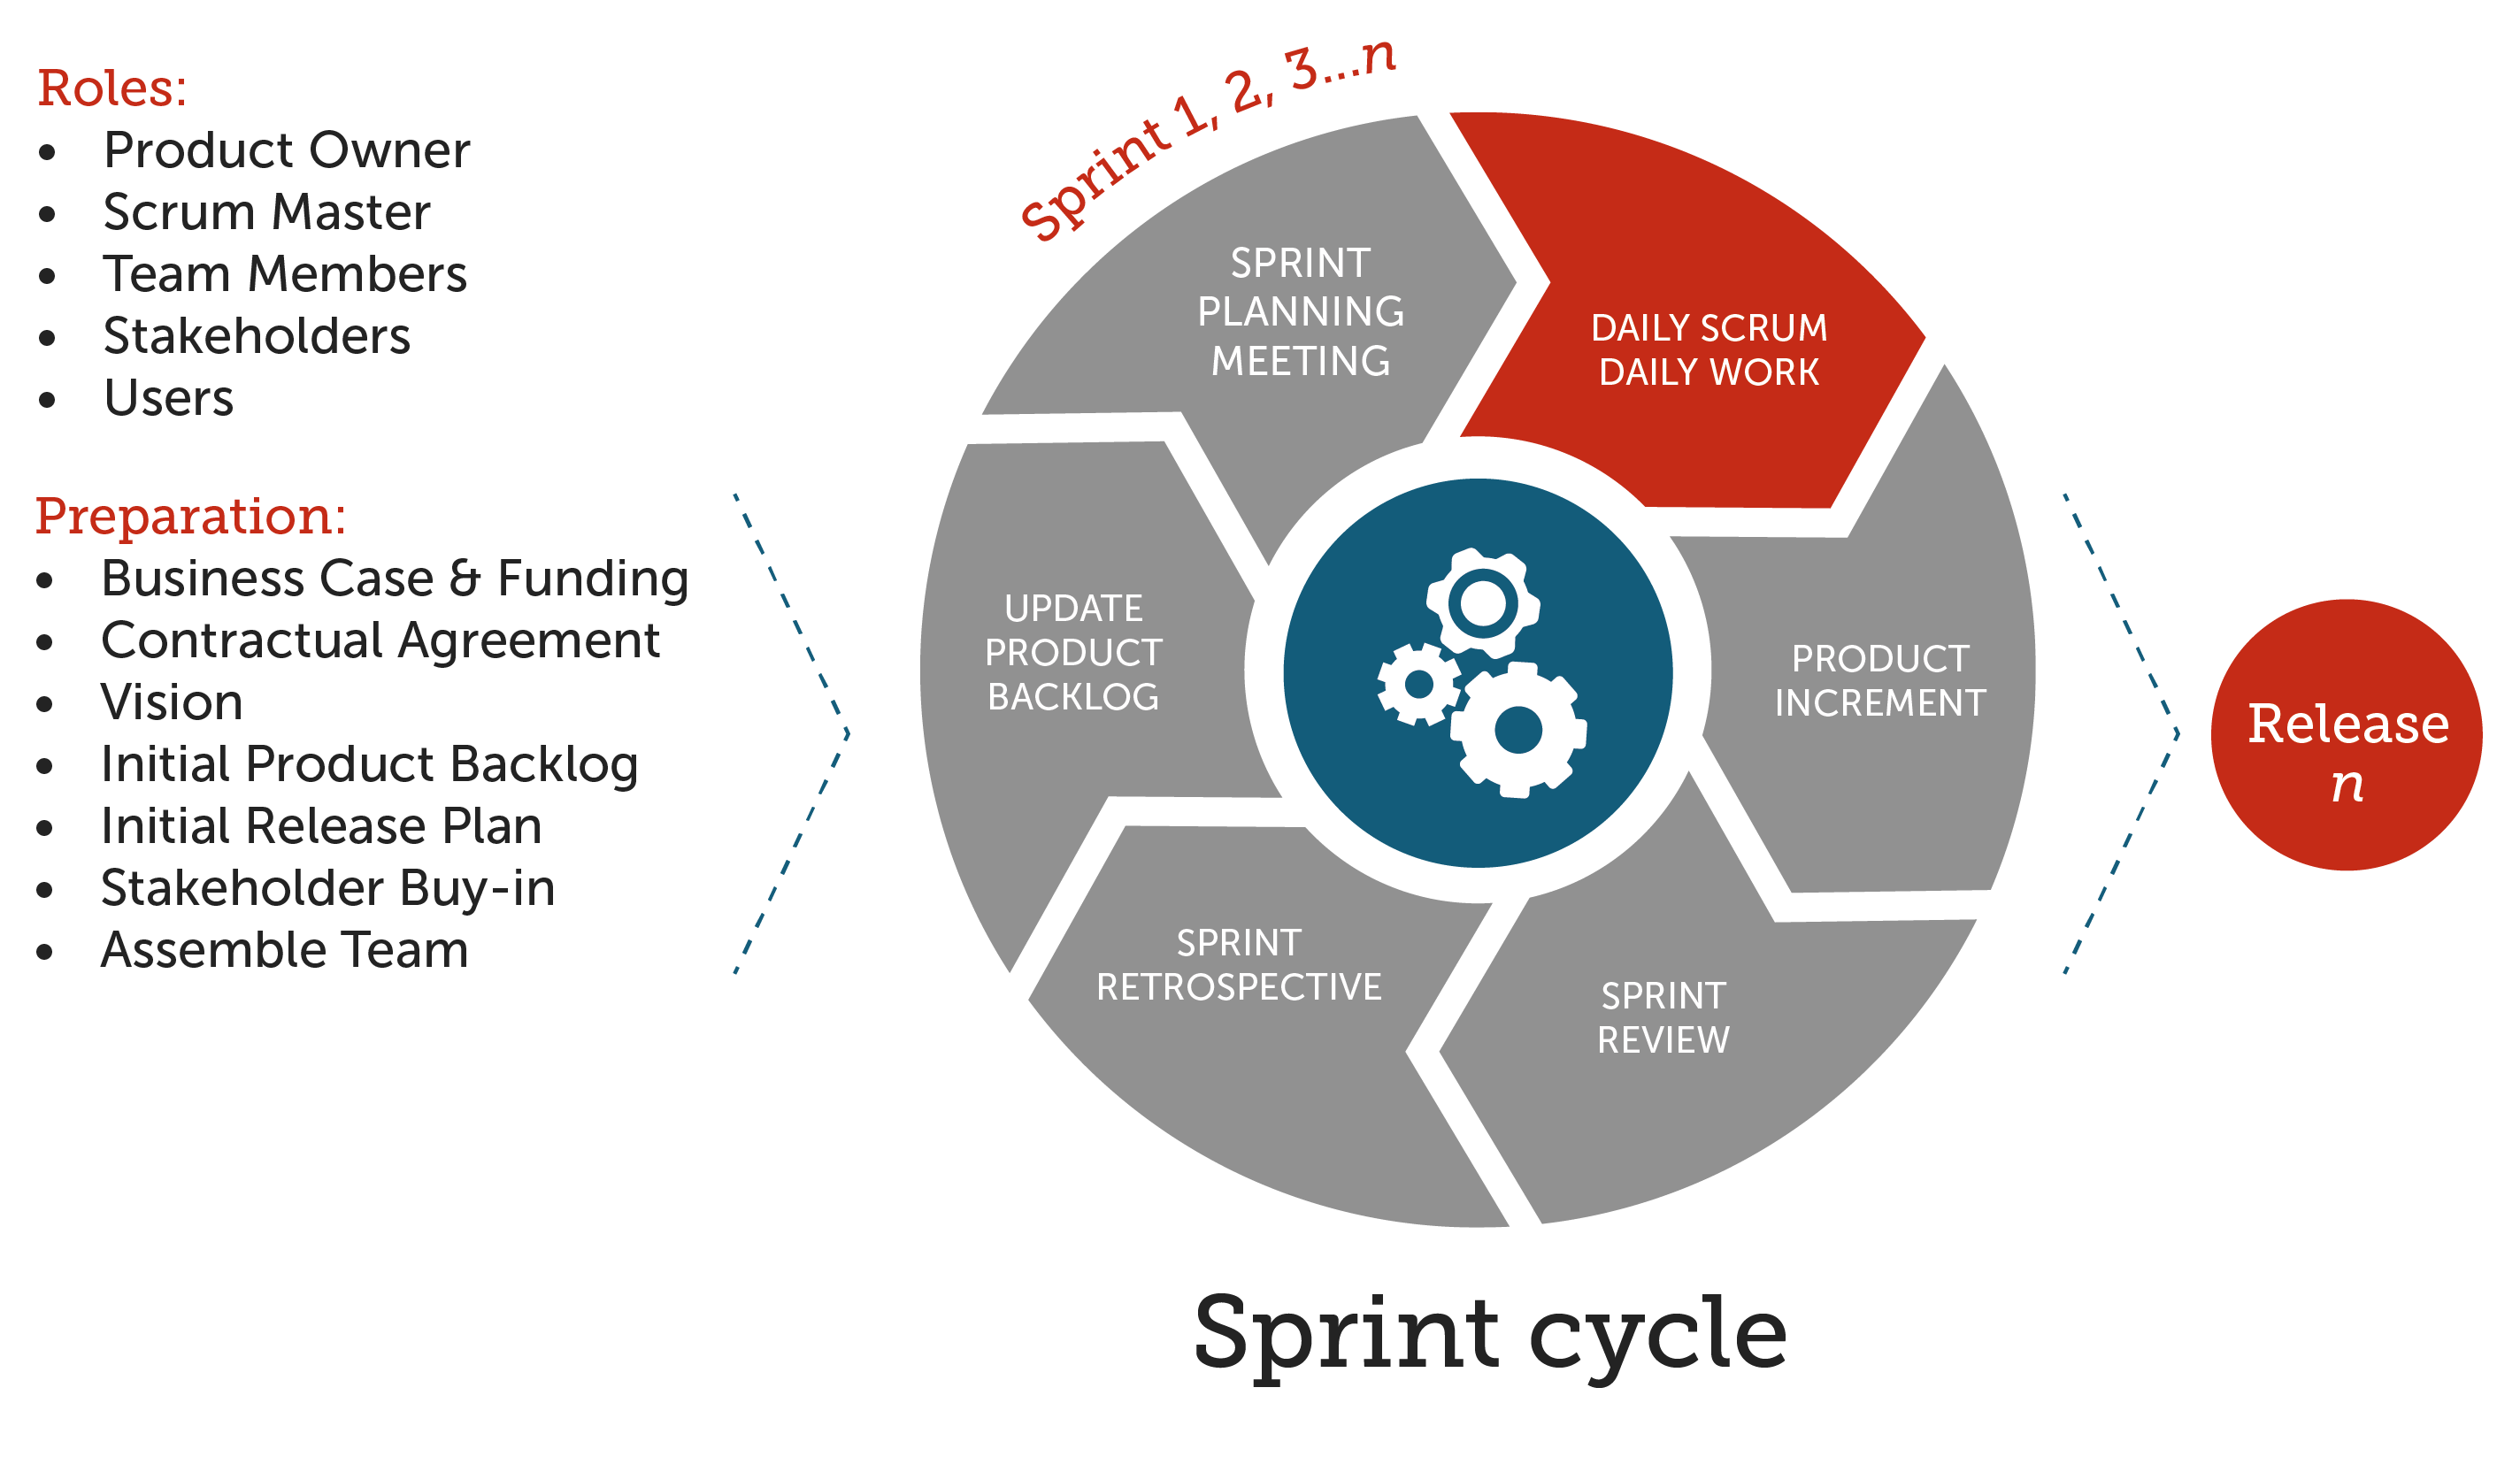
\includegraphics[width=\textwidth,height=0.9\textheight,keepaspectratio]{./images/the-daily-scrum-in-the-sprint-cycle}
  \autocite{ManifestoDigital}
\end{figure}

\section{Größten Vorteile von Scrum}

Agilitaet bedeutet schnell auf Anforderungsaenderung reagieren zu koennen, aber auch schnell Feedback zu diesen Anforderungen geben zu koennen.
Feedback in welcher Form?
Sprint Planning kann genutzt werden zum Adressieren der neuen Anforderungen.
Iterative Natur

People over Tools.
Team wird hervorgehoben bei Scrum.
Nicht einzelne Experten, sondern das gesamte Team steht fuer Qualitaet.
Regel ist, dass jedes Teammitglied zu allem beitragen kann.
Jedes Teammitglied ist in der Lage, sich eine Aufgabe zu schnappen.
Das bedeutet, dass jedes Teammitglied aber auch fuer jedes Stueck Code zustaendig sein kann.
Das erzwingt, dass das ganze Team an einem Strang zieht, oftmals "Whole-Team"-Approach genannt.
Dieser Ansatz ist vorallem wichtig im Bezug auf TDD.
Waehrend TDD kann nur eine angemessene Testbasis geschaffen werden, wenn jeder Entwickler sich verantwortlich fuehlt, neue Tests zu schreiben, aber auch alte Tests zu pflegen.
Neue Anforderungen bedeuten, dass neue Tests geschrieben werden muessen, aber auch, dass eventuell alte Tests angepasst werden muessen.
Kostensparender Entwicklungsprozess
Zerfaellt die Qualitaet der Testsuite, so zerfaellt fuer einer der besten und schnellsten Moeglichkeiten, Feedback bezueglich der Qualitaet zu gewinnen.
  Projekte mit vielen \enquote{moving targets} sind durch Scrum lösbar.
  Iterative Natur bietet Möglichkeit, Software schnell und strukturiert zu entwickeln, um ein Minimum Viable Project zu liefern.
  Kurzen Sprints erlauben, dass Software nicht für Ewigkeiten entwickelt wird, und dann ein falsches Projekt herauskommt.
  Probleme werden schnell identifiziert.
  Planung von Sprint zu Sprint, Team organisiert sich selbst, daher wenig Overhead.
  Nur Features implementiert, die der Kunde explizit fordert

\section{Nachteile}

\begin{itemize}
  \item Nur ein Framework
  \item Kein festes Projektabschlussdatum führt oft zu \enquote{Feature Creep}
  \item Keine festen Softwareentwicklungsphasen innerhalb eines Sprints
  \item Projekterfolg hängt von Kooperation des Teams ab
  \item Erfordert viel Disziplin
  \item Qualität schwer zu gewährleisten:
  \begin{itemize}
    \item Team muss entweder qualifiziert sein oder
    \item Team muss agressiven Testprozess durchführen
  \end{itemize}
\end{itemize}


\chapter{Einbindung von TDD in Scrum}

Barry Boehm (Erfinder des Spiralenmodells) hat Unterschied schön hervorgehoben:
Are we building the product right?
Are we building the right product?

Beides wird durch TDD unterstuetzt beantwortet.

Was bringen Tests?
Instant Feedback bezueglich des Codes, helfen also bei Agilitaet!
Funktioniert der Code, den ich geschrieben habe?
Kann ich den Use Case des Kundens modellieren?
Kann ich nicht-funktionale Anforderungen abdecken?

Tests schwer in schnellen Iterations-Zyklus einzubinden, vor allem, weil keine seperate Testphase gegeben ist, zumindest nicht im tradionellen Scrum-Model.
TDD bedeutet auch, dass Entwickler Tests schreiben; Tests, die automatisiert auszufuehren sind.
Koennen also auch schnell genutzt werden, bei Aenderungen neuer Anforderungen Regressionen zu finden.
Test-Code-Test Cycle darf nicht zu lang sein.

Testing selbst evtl schwer, oftmals keine festen Spezifikationen.
Wie loest man das Problem?
Tests und Code ist einfacher zu schreiben, wenn festere Spezifikationen gegeben sind.
Problem entsteht aus schlechten User Stories, sollte bei guten User Stories also nicht entstehen.
TDD mitigiert allerdings schlechte User Stories, da Entwickler gezwungen ist, sich Gedanken ueber den Code und das Design zu machen, bevor Code in Applikation gelangt.
TDD kann also auch helfen, "Done"-Definitions zu finden.

\section{Teamorganisation}

In der Informatik betrachten wir oftmals nur die Entwicklerseite, allerdings nicht zu vergessen die anderen Stakeholder.
Wer kann was testen?
Was ist mit einer spezifischen Testerroller oder QA?
Sollte ein Programmierer alles alleine testen?
Wie koennen User Stories geloest werden, wo Tester und Programmierer eventuell nicht mit Anforderungen klar kommen?
Kunde involvieren! -> Power of Three.

\section{Developer-TDD + ATDD}

\begin{itemize}
    \item Während Sprint Planning: Benutzeranforderungen als Acceptance Tests schreiben,
    \item Während User Stories: Acceptance Test aufgeteilt in kleinere Unit Tests,
    \item Eigentlicher Programmierprozess beginnt, bis Unit Tests / Acceptance Tests bestehen
\end{itemize}

\begin{figure}[!htb]
    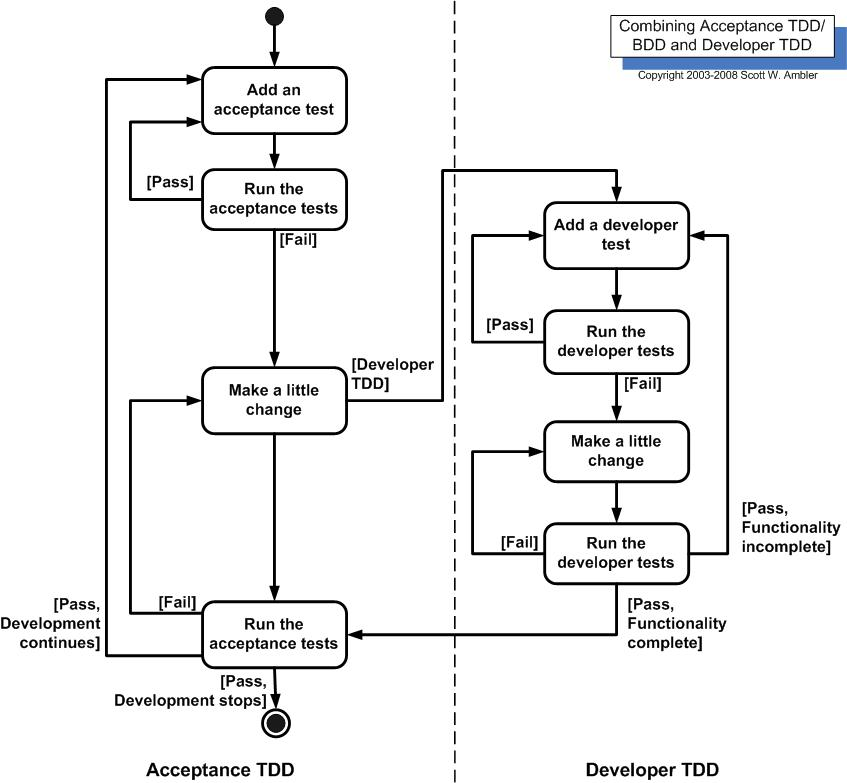
\includegraphics[width=\textwidth,height=0.8\textheight,keepaspectratio]{./images/atdd.jpg}
    \autocite{astels_2003}
\end{figure}

\section{Projektmanagersicht}
\subsection{Zeitmanagement}

Was bedeutet TDD fuer die Estimates?
Lohnt sich Tests schreiben ueberhaupt?
Bedeuten Tests nicht, dass mehr Aufwand gebracht werden muss, "nutzlosen" Code zu produzieren?
Das ist doch eine Reduktion des Throughputs.
Iterationen sind doch eh schon kurz genug.
Wann soll ueberhaupt getestet werden?
Meist Sprints so kurz definiert, dass Entwickler mit Stories fertig werden.
Wenn die Story fertig ist, sollte also Sprint beendet werden.

Stories sollten erst fertig sein, wenn sie vernuenftig getestet sind.
Stories sollten IN dem Sprint getestet werden, in der sie ins Sprint Backlog getan wurden.
Testing in agilen Entwicklungsprozessen sollte nicht designed werden nach dem Konzept, dass Testing auf den letzten Sprint arbeitet.
Immer momentanen Sprint testen, daher auch dafuer Zeit nehmen!

\subsection{Technical Debt}

Hilft TDD evtl technical debt zu mitigieren?

\subsection{Statistiken}

\subsubsection{Wie verifizieren agile Teame ihre Arbeit?}
    \begin{tabularx}{\linewidth}{
      |>{\hsize=0.7\hsize} X |
      >{\hsize=0.2\hsize} X |
      >{\hsize=0.1\hsize} X |
      >{\hsize=0.1\hsize} X |
    }
    \hline
    \textbf{Methodik} & \textbf{2008} & \textbf{2010} & \textbf{2013}\\ \hline
    Iteration demos & - & \textbf{79\%} & 58\% \\ \hline
    Developer regression testing & 60\% & \textbf{71\%} & 49\% \\ \hline
    Developer TDD & \textbf{71\%} & 53\% & 38\% \\ \hline
    Acceptance TDD & 40\% & \textbf{44\%} & 18\% \\ \hline
    All-hands demos & \textbf{56\%} & 42\% & 30\% \\ \hline
    End-of-lifecycle testing & 45\% & 41\% & \textbf{50\%} \\ \hline
    Non-solo development & - & \textbf{39\%} & 34\% \\ \hline
    Static-code analysis & - & 32\% & \textbf{39\%} \\ \hline
    Parallel independent testing & \textbf{36\%} & 26\% & 22\% \\ \hline
    External reviews & \textbf{52\%} & 23\% & 32\% \\ \hline
    Dynamic code analysis & \textbf{23\%} & 21\% & 22\% \\ \hline
    \end{tabularx}

\subsubsection{Welche agile Testmethode waren die schwersten zu erlernen?}
  \begin{tabularx}{\linewidth}{
    |>{\hsize=0.7\hsize} X |
    >{\hsize=0.2\hsize} X |
    >{\hsize=0.1\hsize} X |
    >{\hsize=0.1\hsize} X |
  }
  \hline
  \textbf{Methodik} & \textbf{2009} & \textbf{2012}\\ \hline
  Developer TDD & 37\% & 37\% \\ \hline
  Acceptance TDD & 30\% & 39\% \\ \hline
  \end{tabularx}

Nur 2012:
  \begin{itemize}
    \item Getting all testing done in current sprint: 50\%
    \item Validating non-functional requirements: 33\%
    \item Getting stakeholders/customers involved in testing: 33\%
    \item Getting developers to test their own code: 27\%
    \item Initial Estimate and Schedule: 26\%
    \item Adopting new agile testing tools: 16\%
    \item Learning to test throughout the agile lifecycle: 16\%
  \end{itemize}
  \nocite{Ambysoft.Surveys}

\section{Entwicklersicht}

\printbibliography

% Can be used to add a list of acronyms with their description
%\glsaddall
%\deftranslation{to=German}{Acronyms}{Abkürzungsverzeichnis}
%\deftranslation{to=German}{Glossary}{Glossar}
\printacronyms[title=Abkürzungsverzeichnis,toctitle=Abkürzungsverzeichnis]
\printglossary[type=main]

%\addcontentsline{toc}{chapter}{\listfigurename}
\listoffigures      % Abbildungsverzeichnis

%s\addcontentsline{toc}{chapter}{\listtablename}
% \listoftables       % Tabellenverzeichnis

\end{document}
